% Options for packages loaded elsewhere
\PassOptionsToPackage{unicode}{hyperref}
\PassOptionsToPackage{hyphens}{url}
\PassOptionsToPackage{dvipsnames,svgnames,x11names}{xcolor}
%
\documentclass[
  11pt]{article}

\usepackage{amsmath,amssymb}
\usepackage{iftex}
\ifPDFTeX
  \usepackage[T1]{fontenc}
  \usepackage[utf8]{inputenc}
  \usepackage{textcomp} % provide euro and other symbols
\else % if luatex or xetex
  \usepackage{unicode-math}
  \defaultfontfeatures{Scale=MatchLowercase}
  \defaultfontfeatures[\rmfamily]{Ligatures=TeX,Scale=1}
\fi
\usepackage{lmodern}
\ifPDFTeX\else  
    % xetex/luatex font selection
\fi
% Use upquote if available, for straight quotes in verbatim environments
\IfFileExists{upquote.sty}{\usepackage{upquote}}{}
\IfFileExists{microtype.sty}{% use microtype if available
  \usepackage[]{microtype}
  \UseMicrotypeSet[protrusion]{basicmath} % disable protrusion for tt fonts
}{}
\usepackage{xcolor}
\setlength{\emergencystretch}{3em} % prevent overfull lines
\setcounter{secnumdepth}{5}
% Make \paragraph and \subparagraph free-standing
\makeatletter
\ifx\paragraph\undefined\else
  \let\oldparagraph\paragraph
  \renewcommand{\paragraph}{
    \@ifstar
      \xxxParagraphStar
      \xxxParagraphNoStar
  }
  \newcommand{\xxxParagraphStar}[1]{\oldparagraph*{#1}\mbox{}}
  \newcommand{\xxxParagraphNoStar}[1]{\oldparagraph{#1}\mbox{}}
\fi
\ifx\subparagraph\undefined\else
  \let\oldsubparagraph\subparagraph
  \renewcommand{\subparagraph}{
    \@ifstar
      \xxxSubParagraphStar
      \xxxSubParagraphNoStar
  }
  \newcommand{\xxxSubParagraphStar}[1]{\oldsubparagraph*{#1}\mbox{}}
  \newcommand{\xxxSubParagraphNoStar}[1]{\oldsubparagraph{#1}\mbox{}}
\fi
\makeatother


\providecommand{\tightlist}{%
  \setlength{\itemsep}{0pt}\setlength{\parskip}{0pt}}\usepackage{longtable,booktabs,array}
\usepackage{calc} % for calculating minipage widths
% Correct order of tables after \paragraph or \subparagraph
\usepackage{etoolbox}
\makeatletter
\patchcmd\longtable{\par}{\if@noskipsec\mbox{}\fi\par}{}{}
\makeatother
% Allow footnotes in longtable head/foot
\IfFileExists{footnotehyper.sty}{\usepackage{footnotehyper}}{\usepackage{footnote}}
\makesavenoteenv{longtable}
\usepackage{graphicx}
\makeatletter
\newsavebox\pandoc@box
\newcommand*\pandocbounded[1]{% scales image to fit in text height/width
  \sbox\pandoc@box{#1}%
  \Gscale@div\@tempa{\textheight}{\dimexpr\ht\pandoc@box+\dp\pandoc@box\relax}%
  \Gscale@div\@tempb{\linewidth}{\wd\pandoc@box}%
  \ifdim\@tempb\p@<\@tempa\p@\let\@tempa\@tempb\fi% select the smaller of both
  \ifdim\@tempa\p@<\p@\scalebox{\@tempa}{\usebox\pandoc@box}%
  \else\usebox{\pandoc@box}%
  \fi%
}
% Set default figure placement to htbp
\def\fps@figure{htbp}
\makeatother

\usepackage{graphicx}
\usepackage{bbm}
\usepackage{graphics}
\usepackage{amssymb}
\usepackage{amsmath}
\usepackage[nomarginpar]{geometry}
\usepackage{setspace}
\usepackage{natbib}
\onehalfspacing
\usepackage{lscape}
\usepackage{rotating}
\usepackage[tableposition=top]{caption}
\usepackage{tabularx, calc}
\usepackage{threeparttable}
\usepackage{subfigure}
\usepackage{picinpar}  
\usepackage{longtable}
\usepackage{ae}
\usepackage{float}
\usepackage{morefloats}
\usepackage{palatino}
\usepackage{hyperref}
\usepackage{color}
\usepackage{adjustbox}
\usepackage{booktabs} 
\usepackage{ulem}
\usepackage{kotex}
\usepackage{ragged2e}
\usepackage{changepage}
\usepackage{longtable}

\geometry{left=1.0in,right=1.0in,top=1.0in,bottom=1.0in}
\makeatletter
\@ifpackageloaded{caption}{}{\usepackage{caption}}
\AtBeginDocument{%
\ifdefined\contentsname
  \renewcommand*\contentsname{Table of contents}
\else
  \newcommand\contentsname{Table of contents}
\fi
\ifdefined\listfigurename
  \renewcommand*\listfigurename{List of Figures}
\else
  \newcommand\listfigurename{List of Figures}
\fi
\ifdefined\listtablename
  \renewcommand*\listtablename{List of Tables}
\else
  \newcommand\listtablename{List of Tables}
\fi
\ifdefined\figurename
  \renewcommand*\figurename{Figure}
\else
  \newcommand\figurename{Figure}
\fi
\ifdefined\tablename
  \renewcommand*\tablename{Table}
\else
  \newcommand\tablename{Table}
\fi
}
\@ifpackageloaded{float}{}{\usepackage{float}}
\floatstyle{ruled}
\@ifundefined{c@chapter}{\newfloat{codelisting}{h}{lop}}{\newfloat{codelisting}{h}{lop}[chapter]}
\floatname{codelisting}{Listing}
\newcommand*\listoflistings{\listof{codelisting}{List of Listings}}
\makeatother
\makeatletter
\makeatother
\makeatletter
\@ifpackageloaded{caption}{}{\usepackage{caption}}
\@ifpackageloaded{subcaption}{}{\usepackage{subcaption}}
\makeatother

\usepackage[]{natbib}
\bibliographystyle{econ}
\usepackage{bookmark}

\IfFileExists{xurl.sty}{\usepackage{xurl}}{} % add URL line breaks if available
\urlstyle{same} % disable monospaced font for URLs
\hypersetup{
  pdftitle={Paper Template},
  pdfauthor={Hyoungchul Kim; Author 2},
  pdfkeywords={3 to 6 keywords},
  colorlinks=true,
  linkcolor={cyan},
  filecolor={Maroon},
  citecolor={cyan},
  urlcolor={cyan},
  pdfcreator={LaTeX via pandoc}}


\title{Paper Template}
\author{Hyoungchul Kim \and Author 2}
\date{March 8, 2025}

\begin{document}
\def\spacingset#1{\renewcommand{\baselinestretch}%
{#1}\small\normalsize} \spacingset{1}


%%%%%%%%%%%%%%%%%%%%%%%%%%%%%%%%%%%%%%%%%%%%%%%%%%%%%%%%%%%%%%%%%%%%%%%%%%%%%%

\date{\href{https://hchulkim.github.io}{Link to Latest version}\\ \vspace{1em} Last updated March
8, 2025}
\title{Paper Template}
\author{
Hyoungchul Kim\thanks{The creator. The Wharton School, University of
Pennsylvania.}\\
University of XXX\\
\\Author 2\\
University of WWW\\
}
\maketitle

\bigskip
\bigskip
\begin{abstract}
The text of your abstract.
\end{abstract}

\noindent%
{\it Keywords:} 3 to 6 keywords
\vfill

\newpage
\spacingset{1.2} % DON'T change the spacing!

\section{Introduction}\label{sec-intro}

I will show some examples of things you can easily do in quarto-format.

\subsection{Math}\label{math}

You can easily use latex math format in quarto.

This is in-line math: \(x + y = 7\).

This is display-style math: \[x + y = 7.\]

You can also use begin align style syntax: \begin{align}
  x + y &= 7\\
  t + v &= 10.
\end{align}

\subsection{Figures}\label{figures}

Putting figures is easy in quarto. Use syntax like this:

\begin{figure}

\centering{

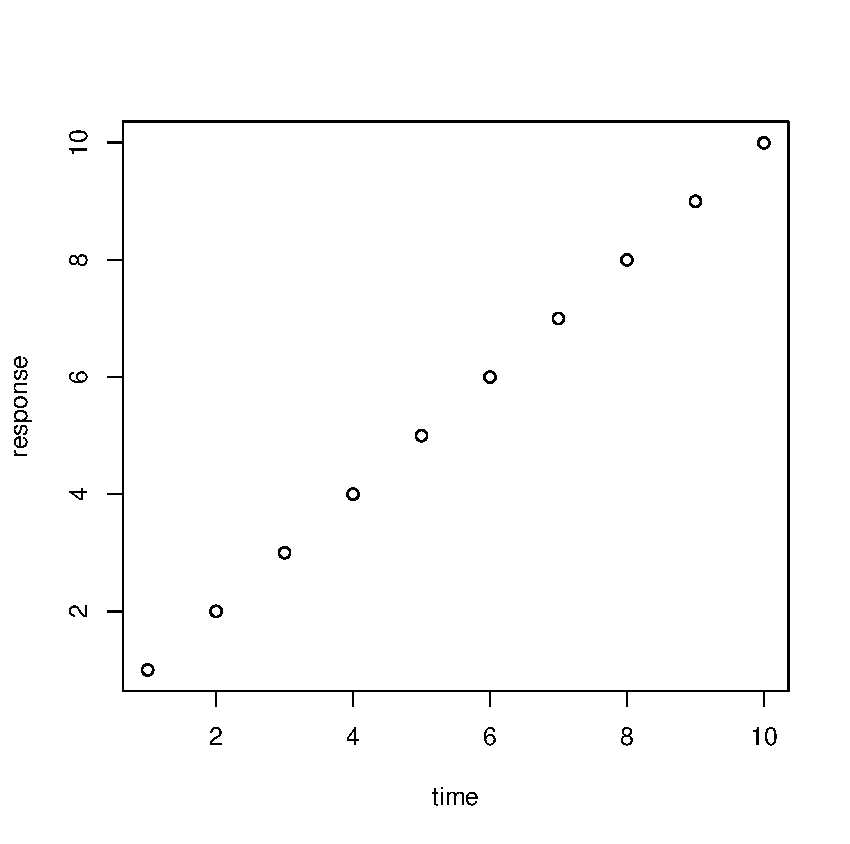
\includegraphics[width=3in,height=\textheight,keepaspectratio]{fig1.pdf}

}

\caption{\label{fig-first}Consistency comparison in fitting surrogate
model in the tidal power example.}

\end{figure}%

\subsection{Tables}\label{tables}

Making custom tables is easy. Do something like this:

\begin{longtable}[]{@{}lllll@{}}
\caption{D-optimality values for design X under five different
scenarios.}\label{tbl-one}\tabularnewline
\toprule\noalign{}
one & two & three & four & five \\
\midrule\noalign{}
\endfirsthead
\toprule\noalign{}
one & two & three & four & five \\
\midrule\noalign{}
\endhead
\bottomrule\noalign{}
\endlastfoot
1.23 & 3.45 & 5.00 & 1.21 & 3.41 \\
1.23 & 3.45 & 5.00 & 1.21 & 3.42 \\
1.23 & 3.45 & 5.00 & 1.21 & 3.43 \\
\end{longtable}

You can also input a table using latex syntax:

\begin{table}[!h] 
  \caption{Main results}\label{tbl-second}
  \resizebox{\textwidth}{!}{
  \centering
\small % Reduce font size
\setlength{\tabcolsep}{4pt} % Adjust column spacing
\begin{tabular}{l *{7}{c}}
\toprule
& $(1)$ & $(2)$ & $(3)$ & $(4)$ & $(5)$ & $(6)$ & $(7)$ \\
\multicolumn{1}{c}{Dependent Variable} & All Waste & Trash & Food & Plastic & Textile & Metal & Can \\
\midrule
$\mathrm{WFH}$ & $-0.039$ & $0.061$ & $-0.110^{**}$ & $0.031^{**}$ & $0.010^{***}$ & $-0.006$ & $-0.010$\\
& $(0.128)$ & $(0.101)$ & $(0.051)$ & $(0.014)$ & $(0.004)$ & $(0.025)$ & $(0.011)$\vspace{1mm} \\
Adjusted $R^2$ & $0.481$ & $0.434$ & $0.475$ & $0.340$ & $0.141$ & $0.307$ & $0.256$\\
$\mathrm{N}$ & $972$ & $972$ & $972$ & $972$ & $972$ & $972$ & $972$\\
\bottomrule
\multicolumn{8}{p{.9\textwidth}}{\small \textbf{Notes.} Standard errors in parentheses are clustered at the district ($N=162$) level. $^{***}~\, \mathrm{p}<~0.01$; $^{**}\, \mathrm{p}< 0.05$ ; $^{*} \, \mathrm{p}<0.10$.}
\end{tabular}}
\end{table}

\begin{itemize}
\tightlist
\item
  Note that figures and tables (such as Figure~\ref{fig-first} and
  Table~\ref{tbl-one}, \ref{tbl-second}) should appear in the paper, not
  at the end or in separate files.
\end{itemize}

\section{Related literature}\label{sec-lit}

Some citation example.

\citet{gelm:veht:2021} offer some guidance about key ideas about
statistical ideas. On an unrelated note, spreadsheets are important to
use correctly \citep{brom:woo:2018}. Log-linear models are an attractive
way to model categorical data \citep{bish:fien:1975}.

\section{Methods}\label{sec-meth}

Lorem ipsum. Lorem ipsum.Lorem ipsum.Lorem ipsum.Lorem ipsum.Lorem
ipsum.Lorem ipsum.Lorem ipsum.Lorem ipsum.Lorem ipsum.Lorem ipsum.Lorem
ipsum.Lorem ipsum.Lorem ipsum.Lorem ipsum.Lorem ipsum.Lorem ipsum.Lorem
ipsum.Lorem ipsum.Lorem ipsum.Lorem ipsum.Lorem ipsum.Lorem ipsum.Lorem
ipsum.Lorem ipsum.Lorem ipsum.Lorem ipsum.Lorem ipsum.Lorem ipsum.Lorem
ipsum.Lorem ipsum.Lorem ipsum.Lorem ipsum.Lorem ipsum.Lorem ipsum.Lorem
ipsum.Lorem ipsum.Lorem ipsum.Lorem ipsum.Lorem ipsum.Lorem ipsum.Lorem
ipsum.Lorem ipsum.Lorem ipsum.Lorem ipsum.Lorem ipsum.Lorem ipsum.Lorem
ipsum.Lorem ipsum.Lorem ipsum.Lorem ipsum.Lorem ipsum.Lorem ipsum.Lorem
ipsum.Lorem ipsum.Lorem ipsum.Lorem ipsum.Lorem ipsum.Lorem ipsum.Lorem
ipsum.Lorem ipsum.Lorem ipsum.Lorem ipsum.Lorem ipsum.Lorem ipsum.Lorem
ipsum.Lorem ipsum.Lorem ipsum.Lorem ipsum.Lorem ipsum.Lorem ipsum.Lorem
ipsum.Lorem ipsum.Lorem ipsum.Lorem ipsum.Lorem ipsum.Lorem ipsum.Lorem
ipsum.Lorem ipsum.Lorem ipsum.Lorem ipsum.

Lorem ipsum.Lorem ipsum.Lorem ipsum.Lorem ipsum.Lorem ipsum.Lorem
ipsum.Lorem ipsum.Lorem ipsum.Lorem ipsum.Lorem ipsum.Lorem ipsum.Lorem
ipsum.Lorem ipsum.Lorem ipsum.Lorem ipsum.Lorem ipsum.Lorem ipsum.Lorem
ipsum.Lorem ipsum.Lorem ipsum.Lorem ipsum.Lorem ipsum.Lorem ipsum.Lorem
ipsum.Lorem ipsum.Lorem ipsum.Lorem ipsum.Lorem ipsum.Lorem ipsum.Lorem
ipsum.Lorem ipsum.Lorem ipsum.Lorem ipsum.Lorem ipsum.Lorem ipsum.Lorem
ipsum.Lorem ipsum.Lorem ipsum.Lorem ipsum.Lorem ipsum.Lorem ipsum.Lorem
ipsum.Lorem ipsum.Lorem ipsum.Lorem ipsum.Lorem ipsum.Lorem ipsum.Lorem
ipsum.Lorem ipsum.Lorem ipsum.Lorem ipsum.Lorem ipsum.Lorem ipsum.Lorem
ipsum.Lorem ipsum.Lorem ipsum.Lorem ipsum.Lorem ipsum.Lorem ipsum.Lorem
ipsum.Lorem ipsum.Lorem ipsum.Lorem ipsum.Lorem ipsum.Lorem ipsum.Lorem
ipsum.Lorem ipsum.Lorem ipsum.Lorem ipsum.Lorem ipsum.Lorem ipsum.Lorem
ipsum.Lorem ipsum.Lorem ipsum.

Lorem ipsum.Lorem ipsum.Lorem ipsum.Lorem ipsum.Lorem ipsum.Lorem
ipsum.Lorem ipsum.Lorem ipsum.Lorem ipsum.Lorem ipsum.Lorem ipsum.Lorem
ipsum.Lorem ipsum.Lorem ipsum.Lorem ipsum.Lorem ipsum.Lorem ipsum.Lorem
ipsum.Lorem ipsum.Lorem ipsum.Lorem ipsum.Lorem ipsum.Lorem ipsum.Lorem
ipsum.Lorem ipsum.Lorem ipsum.Lorem ipsum.Lorem ipsum.Lorem ipsum.Lorem
ipsum.Lorem ipsum.Lorem ipsum.Lorem ipsum.Lorem ipsum.Lorem ipsum.Lorem
ipsum.Lorem ipsum.Lorem ipsum.Lorem ipsum.Lorem ipsum.Lorem ipsum.Lorem
ipsum.Lorem ipsum.Lorem ipsum.Lorem ipsum.Lorem ipsum.Lorem ipsum.Lorem
ipsum.Lorem ipsum.Lorem ipsum.Lorem ipsum.Lorem ipsum.Lorem ipsum.Lorem
ipsum.Lorem ipsum.Lorem ipsum.Lorem ipsum.Lorem ipsum.Lorem ipsum.Lorem
ipsum.Lorem ipsum.Lorem ipsum.Lorem ipsum.Lorem ipsum.Lorem ipsum.Lorem
ipsum.Lorem ipsum.Lorem ipsum.Lorem ipsum.Lorem ipsum.Lorem ipsum.Lorem
ipsum.Lorem ipsum.Lorem ipsum.Lorem ipsum.Lorem ipsum.Lorem ipsum.Lorem
ipsum.Lorem ipsum.Lorem ipsum.Lorem ipsum.

\section{Results}\label{sec-result}

\section{Conclusion}\label{sec-conc}

\phantomsection\label{appendix}
\bigskip

\begin{center}

{\large\bf APPENDIX}

\end{center}

Section for Appendix.

\section{BibTeX}\label{bibtex}

We encourage you to use BibTeX. If you have, please feel free to use the
package natbib with any bibliography style you're comfortable with. The
.bst file agsm has been included here for your convenience.


  \bibliography{bibliography.bib}



\end{document}
